\section{Denotations}\label{sec:denote}

\subsection{Overview}


Concurrent programs are a mix of control constructs ($\cseq,\parallel,+,\dots$)
and atomic actions $a$ that modify \emph{program state} $s$.
This is all that is visible to the programmer.



Our denotational UTP semantics
is inspired by that done for UTPP\cite{DBLP:conf/icfem/WoodcockH02},
itself based on a UTP theory of \emph{action systems}.
First, we add a new state component, not visible in the program text,
which is a set of labels ($ls$).
These labels are used to orchestrate the flow of control.
Given an atomic action $a$ that only knows about program state $s$,
we use notation $\catom a$ to describe a lifted version
of $a$ that takes account of the contents of the label-set $ls$.
In effect a lifted atomic state action is disabled until
a particular label is present in that set.
A disabled action does not modify the state any way
and simply monitors the label-set.
Once an action observes the presence/arrival of its label,
it then becomes active.
An active lifted action $\catom a$ atomically modifies the extended state as follows:
\begin{itemize}
  \item It makes the changes to $s$ as determined by its underlying action $a$.
  \item It removes the enabling label from the label-set.
  \item It adds in appropriate ``continuation'' labels to $ls$.
\end{itemize}
In \cite{DBLP:conf/icfem/WoodcockH02},
the language syntax required explicit (starting) labels
for every atomic state change action,
and these are used as lifted action enablers.
The continuation labels were taken to the the enabling labels
of whatever other actions occurred immediately after, in the program.
This means that the resulting semantics is not compositional.

The approach we adopt is to adopt the notion of \emph{label generators}
to create the labels, so ensuring they are unique,
but in such a way as make the generation a compositional process.
In addition we explicitly associate two labels with every program construct:
one that marks the entry into the construct,
and another that indicates the exit.

\subsubsection{On Notation}

We make liberal use of a number of shorthand notations,
largely to reduce expression size and clutter.
Typically these reduce the use of infix operators,
and in one notable case, collapse large conjunctions
of implications into a simple form with string visual cues.
Each shorthand is introduced by a subsection similar to this one.

\subsection{Label Generation}

INTRODUCE

\RLEQNS{
   g &:& Gen = \setof g  & \mbox{only one variable!}
\\ \ell &:& Gen \fun Lbl
\\ G \in Gen &::=&  g     & \mbox{the ``root'' generator}
\\           &\mid& G_{:} & \mbox{resulting generator after label produced}
\\           &\mid& G_1   & \mbox{first generator after generator split}
\\           &\mid& G_2   & \mbox{second generator after generator split}
\\ L \in Lbl &::=& \ell_G & \mbox{label produced by generator}
}
Note that our generator expression language has only one variable, $g$,
which denotes the ``root'' generator.
All generator expressions have the form $g$ followed by zero
or more uses of $:$, $1$ and $2$.
We say the  ``root'' generator because this notion is local to a
particular context, and we can relativise things by replacing $g$
by an arbitrary $G$ expression.
We define the notion of the set of labels produced by a generator,
which must satisfy the following laws:
\RLEQNS{
   labs &:& Gen \fun \power Lbl
\\ labs(G) &=& \setof{\ell_G} \cup labs(G_{:}) \cup labs(G_1) \cup labs(G_2)
  &\elabel{labs-def}
\\ \ell_G &\notin& labs(G_{:})
   &\elabel{labs-unique}
\\ \emptyset &=& labs(G_1) \cap labs(G_2)
  &\elabel{labs-split-disjoint}
}
The conceptually simplest model of such a generator
is one where labels are simply the strings of $:$, $1$ and $2$
that designate how its generator was produced from the root.
With this model we also get the following law:
For any generator expression $G$,
the following four sets are mutually disjoint:
\[
  \setof{\ell_G}
  \quad
  labs(G_{:})
  \quad
  labs(G_1)
  \quad
  labs(G_2)
  \qquad
  \elabel{labs-fully-disjoint}
\]

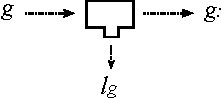
\includegraphics{images/new-label}

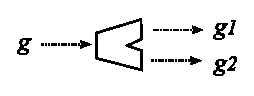
\includegraphics{images/split-gen}


\subsection{Observation Variables}

\begin{eqnarray*}
   s, s' &:& \mathcal S
\\ ls, ls' &:& \mathcal P (Lbl)
\\ g &:& Gen
\\ in, out &:& Lbl
\end{eqnarray*}
We assume a general notion of expressions ($e$)
and say that an expression $e$ is ``ground''
if it's free variables are limited to only $g$, $in$ and $out$.


\subsection{Label-Set Invariants}


We want to be able to specify that certain combinations
of labels should never appear simultaneously
in the global label set ($ls$).
We do this by defining a label-set invariant $I$
which has alphabet $ls,in,out,g$.

We start by defining a general abstract way of specifying
sets with valid combinations
of values drawn from a parameter type $\tau$.
\RLEQNS{
   i \in I_\tau &::=& \tau   &  \mbox{can contain this value}
\\ &\mid& \otimes(i,\ldots,i) & \mbox{at most one of these allowed to contain}
\\ &\mid& \cup (i,\ldots,i) & \mbox{any of these allowed to contain}
}

We define what it means for an atomic action invocation
to satisfy an invariant parameterised on the label type ($Lbl$).
\RLEQNS{
  ls \textbf{ lsat } I \land A(E|a|N) &\implies& ls' \textbf{ lsat } I
}
We can re-formulate this as a following equivalent test:
\RLEQNS{
   A(E|a|N) \textbf{ sat } I_{Lbl}
   &\defs&
   E \textbf{ lsat } I_{Lbl} \land N \textbf{ lsat } I_{Lbl}
}
In effect we identify the occurrences of labels within this $I$-structure,
and then check the multiplicity constraints:
\RLEQNS{
   L \textbf{ lsat } I_{Lbl} &\defs& res=ok
\\ \textbf{where} && (res,\_) = occChk (occ_L I_{Lbl})
}
The $occ$ function takes a set $L$ of $\tau$ and an $I_\tau$ and returns a $I_\Bool$
that records if the corresponding element of $\tau$ is present in $L$.
\RLEQNS{
   occ &:& \power \tau \fun I_\tau \fun I_\Bool
\\ occ_L~\ell &\defs& \ell \in L
\\ occ_L~\otimes(i_1,\ldots,i_n)
   &\defs&
   \otimes(occ_L~i_1,\ldots,occ_L~i_n)
\\ occ_L~\cup(i_1,\ldots,i_n)
   &\defs&
   \cup(occ_L~i_1,\ldots,occ_L~i_n)
}
The $occChk$ function pattern matches across the boolean values to see if
constraints are satisfied.
The first component of the result is an overall ok/fail indicator,
while the second boolean component indicates if values are present
in any component.
\RLEQNS{
   occChk &:& I_\Bool \fun (\setof{ok,fail}\times \Bool)
\\ occChk(b) &\defs& (ok,b)
\\ occChk(\cup(i_1,\ldots,i_n))
   &\defs&
   (fail,\_),
   \textbf{ if }\exists j @ occChk(i_j) = (fail,\_)
\\ && (ok,b_1 \lor \dots \lor b_n),
   \textbf{ if }\forall j @ occChk(i_j) = (ok,b_j)
\\ occChk(\otimes(i_1,\ldots,i_n))
   &\defs&
   (fail,\_),
   \textbf{ if }\exists j @ occChk(i_j) = (fail,\_)
\\&& (fail,\_) \mbox{ if more than one $(ok,true)$}
\\&& (ok,false) \mbox{ if all are $(ok,false)$}
\\&& (ok,true) \mbox{ if  exactly one $(ok,true)$}
}
We note, as a consequence of the above definitions, that
\RLEQNS{
  \emptyset &  \textbf{lsat} &  I & \elabel{emp-lsat-I}
}
for any label-set invariant $I$.

We introduce a shorthand for invariants illustrated as follows.
\RLEQNS{
  ~ [ a,b,c | d,e | f ]
   &=&
   ls \textbf{ lsat } \otimes(\cup(a,b,c),\cup(d,e),f)
\\ ~[ a | (b|c),(d|e) | f ]
  &=&
  ls \textbf{ lsat } \otimes(a,\cup(\otimes(b,c),\otimes(d,e)),f)
}
In effect we make the involvement of $ls$ implicit,
and use bar ($|$) and comma ($,$) to replace $\otimes$ and $\cup$ respectively.
We also have a shorthand that just denotes
the non-intersecting nature of the arguments.
E.g.,
$\setof{A|B|C}$ asserts that $A$, $B$ and $C$ are mutually disjoint,
without any reference to $ls$ or any other set.

\subsubsection{Invariant Examples}

The following examples show how various instances of $ls \textbf{ lsat } I$
get expanded:
\RLEQNS{
   ~[in|out]
   &=&
   \setof{in} \cap \setof{out} = \emptyset
\\ &\land&
  \setof{in} \subseteq ls \implies \setof{out}\cap ls = \emptyset
\\ &\land&
  \setof{out} \subseteq ls \implies \setof{in}\cap ls = \emptyset
\\
\\ ~[in|\ell|out]
   &=&
   \setof{in} \cap \setof{\ell,out} = \emptyset
\\ &\land&
   \setof{\ell} \cap \setof{in,out} = \emptyset
\\ &\land&
   \setof{out} \cap \setof{in,\ell} = \emptyset
\\ &\land&
  \setof{in} \subseteq ls \implies \setof{\ell,out}\cap ls = \emptyset
\\ &\land&
  \setof{\ell} \subseteq ls \implies \setof{in,out}\cap ls = \emptyset
\\ &\land&
  \setof{out} \subseteq ls \implies \setof{in,\ell}\cap ls = \emptyset
\\
\\ ~[ a | (b|c),(d|e) | f ]
   &=&
   \setof{a} \cap \setof{b,c,d,e,f} = \emptyset
\\ &\land&
   \setof{b,c,d,e} \cap \setof{a,f} = \emptyset
\\ &\land&
   \setof{f} \cap \setof{a,b,c,d} = \emptyset
\\ &\land&
  \setof{a} \subseteq ls \implies \setof{b,c,d,e,f}\cap ls = \emptyset
\\ &\land&
  \setof{b,c,d,e} \subseteq ls \implies \setof{a,f}\cap ls = \emptyset
\\ &\land&
  \setof{f} \subseteq ls \implies \setof{a,b,c,d,e}\cap ls = \emptyset
\\ &\land&
   \setof{b} \cap \setof{c} = \emptyset
\\ &\land&
   \setof{d} \cap \setof{e} = \emptyset
\\ &\land&
  \setof{b} \subseteq ls \implies \setof{c}\cap ls = \emptyset
\\ &\land&
  \setof{c} \subseteq ls \implies \setof{b}\cap ls = \emptyset
\\ &\land&
  \setof{d} \subseteq ls \implies \setof{e}\cap ls = \emptyset
\\ &\land&
  \setof{e} \subseteq ls \implies \setof{d}\cap ls = \emptyset
}
Here one of $b$ or $c$ may occur in $ls$ along with one of  $d$ or $e$.
In this theory,
we use the label generators to ensure that the disjointness
conditions of the invariants are always true, by construction.

\subsubsection{Notation}

\RLEQNS{
   ls(\ell) &\defs& \ell \in ls
\\ ls(L) &\defs& L \subseteq ls
\\ ls(\B\ell) &\defs& \ell \notin ls
\\ ls(\B L) &\defs& L \cap ls = \emptyset
}



\subsection{``Standard'' UTP Predicates}

INTRODUCE

\RLEQNS{
   P \cond C Q
   &\defs&
   C \land P \lor \lnot C \land Q
   & \elabel{UTP-cond-def}
\\ \Skip
   &\defs&
   s'= s \land ls'=ls
   & \elabel{UTP-skip-def}
\\ P \seq Q
   &\defs& \exists s_m,ls_m \bullet
\\ && \qquad P[s_m,ls_m/s',ls'] \land Q[s_m,ls_m/s,ls]
   & \elabel{UTP-seq-def}
\\ C * P
   &=&
   P ; C * P \cond C \Skip
   & \elabel{UTP-loop-unroll}
}
We also define a specialised form of sequential composition
to be used when neither component refers to $ls$ or $ls'$,
and its unit:
\RLEQNS{
   P \seq_s Q
   &\defs&
   \exists s_m \bullet P[s_m/s'] \land Q[s_m/s]
   & \elabel{UTP-s-seq-def}
\\ ii &\defs& s'=s & \elabel{ii-def}
}
Note that if neither predicate mentions $ls$ or $ls'$
then the effect of $\seq$ and $\seq_s$ is the same.
We often omit the $s$ subscript when its use is clear from context.

\subsection{Healthiness Conditions}

\subsubsection{Disjoint Labels}

We have a general healthiness condition (Disjoint Labels) which asserts
that the labels associated with $in$, $out$ and $g$
are different:
\RLEQNS{
  \DL(P) &=& P \land in \neq out \land \setof{in,out} \cap labs(g) = \emptyset
}

\subsubsection{Wheels-within-Wheels}

The key intuition behind this compositional semantics was to take the
$run$ function of the action-system based semantic model used in UTPP,
and drive it inwards to every level of the program.
The original $run$ can be defined in the context of this theory as
\[
  run(P) = ls := \setof{in} ; \lnot (out \in ls) * P
\]
However this failed to keep atomic components ``live''.
They could never be re-executed,
as would be required if they were within an iteration.
Instead it was realised that every construct (atomic and composite)
would have to be within an infinite loop.
\RLEQNS{
   \W(P) &\defs& \true * P &\elabel{W-as-loop}
}
This bold step turns out to be remarkably effective,
with some quite counter-intuitive outcomes.
However it does depend on a specific tweak to the
definition of an atomic action.
In effect we define an atomic action
as placing a basic action inside such a loop,
but within a non-deterministic choice between it
and a \emph{stuttering} step, denoted by UTP skip:
\RLEQNS{
  \catom a &\defs& \W(\Skip \lor A(in|a|out))
}
A result of this is that this stuttering step gets
propagated up to enclosing composites,
so in effect we see $\W(C)=\W(\Skip\lor C)$
where $C$ is any predicate denoting the semantics of a command.
We give more details about this in the section on calculation (\S\ref{sec:calc}).
One key calculational advantage of this is that we can rewrite
the rhs of the definition of $\W$ as:
\RLEQNS{
   \W(P) &  =  & \bigvee_{i \in 0,\dots} \Skip \seq P^i &\elabel{W-as-NDC}
}%
We note explicitly here that, in effect,
our semantic model is based on unbounded non-determinism.

However, for iteration-free programs
we find that there is a finite $k$ such that $P^k = \false$,
in which case the non-determinism is bounded.
We get these finite results that seem very similar
to the results obtained by using $run$ above.
Using $run$ results in predicates that cannot be composed
to get composite behaviour.
However, using $\W$ results in a slight variation,
which is composable!
What turns out to be crucial
to this outcome is the explicit stuttering option in the infinite loop.

\subsubsection{Mumble Closure}

A program's semantics includes all its mumblings,
and so should be unchanged if sequentially composed with itself
using \emph{UTP} sequential composition:
\RLEQNS{
   P \seq P &=& P  & \eref{mumble-closure}
}

\subsection{UTP Denotational Semantics}

INTRODUCE

We present each construct individually,
with full diagrams for each \dots



\subsubsection{Basic Action}

Basic Action $A(E|a|N)$ is enabled when all the labels in $E$
are present in the global label-set
and atomic action $a$ does not evaluate to $\false$
in the current program state.
If so enabled,  it performs action $a$, removes the labels in $E$
from the label-set, and adds in those in $N$.
\RLEQNS{
   A(E|a|N)
   &\defs&
   ls(E) \land a \land ls'=(ls\setminus E) \cup N
   & \elabel{A-def}
}




\newpage
\subsubsection{Atomic Action}

\RLEQNS{
  \catom a
  &\defs& [in|out] \land \W(\Skip \lor A(in|a|out)) & \elabel{sem:atomic}
\\ &=&  [in|out] \land (\Skip \lor A(in|a|out))
        & \elabel{nf-atomic}
}
\includegraphics{images/atomic-action}


\subsubsection{Guarded Atomic Action}
In effect there is no real difference between $c \pgrd a$
and $\true \pgrd (c \land a)$,
so in fact we don't need guarded actions as basic.
This is an advantage of treating the atomic action as a relational predicate
on state.

\RLEQNS{
 c \pgrd a &\defs& \catom{c \land a}  &\elabel{sem:pgrd}
}


\subsubsection{Skip}

\RLEQNS{
   ii     &\defs& s'=s
\\ \cskip &\defs& \catom{ii}  &\elabel{sem:skip}
\\  &=&  [in|out] \land (\Skip \lor A(in|ii|out))
    &\elabel{nf-skip}
}

\newpage
\subsubsection{Sequential Composition}

\RLEQNS{
   P \cseq Q
   &\defs&
   [in|\ell_g|out]\land \W(P[g_{:1},\ell_g/g,out] \lor Q[g_{:2},\ell_g/g,in])
   & \elabel{sem:seq}
}
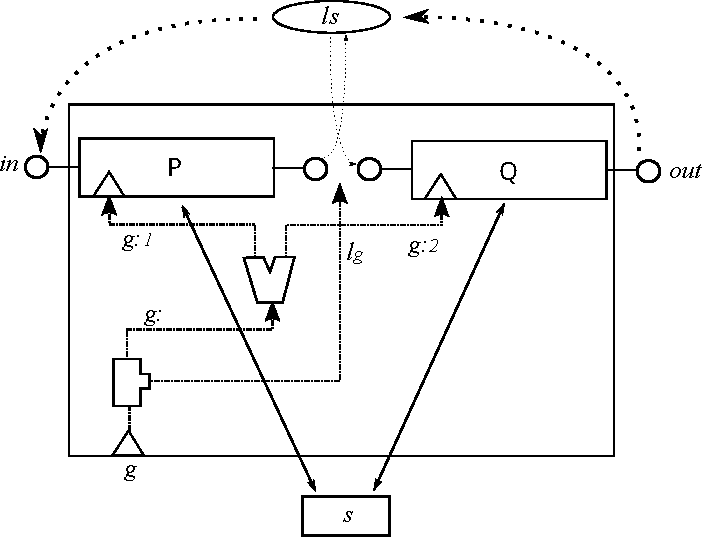
\includegraphics{images/seq-comp-actual}

\newpage
\subsubsection{Parallel Composition}

\RLEQNS{
   P \parallel Q
   &\defs&
   [in|(\ell_{g1}|\ell_{g1:}),(\ell_{g2}|\ell_{g2:})|out] \land {}
   & \elabel{sem:par}
\\&& \W(\quad\phlor A(in|ii|\ell_{g1},\ell_{g2})
\\ && \qquad {}\lor
   P[g_{1::},\ell_{g1},\ell_{g1:}/g,in,out]
\\ && \qquad {}\lor
    Q[g_{2::},\ell_{g2},\ell_{g2:}/g,in,out]
\\ && \qquad {}\lor
   A(\ell_{g1:},\ell_{g2:}|ii|out)~)
}

\includegraphics{images/parallel-label-gen}

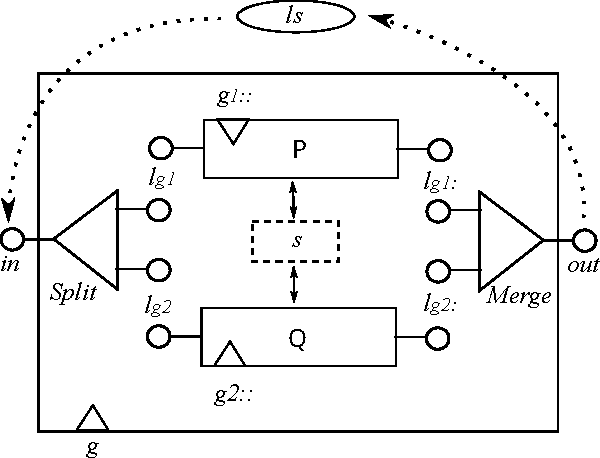
\includegraphics{images/par-comp-actual}


\newpage
\subsubsection{Nondeterministic Choice}

\RLEQNS{
   P + Q
   &\defs&
   [in|\ell_{g1}|\ell_{g2}|out] \land {}
   & \elabel{sem:NDC}
\\ && \W(\quad {}\phlor A(in|ii|\ell_{g1})
\\ && \qquad {} \lor
                     A(in|ii|\ell_{g2})
\\ && \qquad {} \lor
   P[g_{1:},\ell_{g1}/g,in]
\\ && \qquad {} \lor
   Q[g_{2:},\ell_{g2}/g,in]~)
}

\subsubsection{Nondeterministic Loop}


\RLEQNS{
   P^*
   &\defs&
   [in|\ell_g|out] \land {}
   & \elabel{sem:star}
\\ && \W(\quad  \phlor A(in|ii|out)
\\ && \qquad {}\lor A(in|ii|\ell_g)
\\ && \qquad {}\lor P[g_{:},\ell_g,in/g,in,out]~)
}

\newpage
\subsubsection{Conditional Choice}

\RLEQNS{
   P \dcond c Q
   &\defs&
   [in|\ell_{g1}|\ell_{g2}|out] \land {}
   & \elabel{sem:cond}
\\ && \W(\quad {}\phlor A(in|c \land ii|\ell_{g1})
\\ && \qquad {} \lor
                     A(in|\lnot c \land ii|\ell_{g2})
\\ && \qquad {} \lor
   P[g_{1:},\ell_{g1}/g,in]
\\ && \qquad {} \lor
   Q[g_{2:},\ell_{g2}/g,in]~)
}

\includegraphics{images/conditional-actual}

\newpage
\subsubsection{Conditional Loop}


\RLEQNS{
   c \ddo P
   &\defs&
   [in|\ell_g|out] \land {}
   & \elabel{sem:iter}
\\ && \W(\quad  \phlor A(in|\lnot c \land ii|out)
\\ && \qquad {}\lor A(in|c \land ii|\ell_g)
\\ && \qquad {}\lor P[g_{:},\ell_g,in/g,in,out]~)
}

\includegraphics{images/iteration-actual}

\newpage
\subsection{Essential Properties?}

Looking forward we will want some key algebraic properties:
\RLEQNS{
   ~[S_1|\dots|S_n]
   &=&
   [S_{\rho(1)}|\dots|S_{\rho(n)}]
\\ && \rho \textrm{ a permutation of } 1\dots n
\\ ~[S_1|\dots|S_i|S_{i+1}|\dots|S_n]
   &\implies&
   [S_1|\dots|S_i]
   ,\quad i > 1 &\elabel{I-subsumption}
\\ ~[S_1|\dots|S_n]\gamma &=& [S_1\gamma|\dots|S_n\gamma]
   & \elabel{I-gamma-subst}
\\ A(E|a|N)\gamma &=& A(E\gamma|a|N\gamma)
\\ A(E|a|N) \textbf{ sat } I
   &=&
   A(E|a|N)\gamma \textbf{ sat } I\gamma
   , \quad \mbox{arbitrary }\gamma
\\ ((ls\setminus R)\cup A)(S)
   &=&
   ls(F(R,A,S)) \land P(R,A,S)
\\ \Skip \seq P &=~P~=& P \seq \Skip
\\ (P\seq Q)\gamma &=& P\gamma \seq Q\gamma  & \elabel{seq-gnd-distr}
\\ \Skip\gamma &=& \Skip
\\ \DL(P) && \textrm{monotonic in } P
\\ \DL(\DL(P)) &=& \DL(P)
\\ \DL(P\gamma) &=& P\gamma
\\ \W(P)  && \textrm{monotonic in } P
\\ \W(\W(P)) &=& \W(P) & ?
\\ \W(\W(\Skip \lor P)) &=& \W(\Skip \lor P)
\\ \W(\Skip \lor P) &=& \bigvee_{i \in 0,\dots} \Skip \seq P^i
   & \elabel{W-as-NDC}
\\ \W(P)\gamma &=& \W(P\gamma) & \elabel{W-gamma-subst}
\\ \W(\Skip \lor P) &=& \Skip \lor \W(\Skip \lor P)
\\ I \land \W(P) &=& \W(I \land P) & \elabel{I-W-distr}
}

When $P\gamma$ executes:
\begin{description}
  \item[\elabel{P-removes-in}]
    it will remove $in\gamma$ from $ls$ at some point;
  \item[\elabel{P-removes-g}]
    the only other labels it removes are in $labs(g\gamma)$;
  \item[\elabel{P-adds-out}]
    it adds $out\gamma$ into $ls$ at some point;
  \item[\elabel{P-adds-g}]
    the only other labels it adds are in $labs(g\gamma)$;
  \item[\elabel{P-ignores-rest}]
    and its behaviour is not affected by any label not
    in
    \\$\setof{in\gamma,out\gamma} \cup labs(g\gamma)$.
\end{description}
We can summarise this as follows:
\begin{itemize}
  \item $P\gamma$ actions are enabled by labels in $in\gamma,g\gamma$
  \item $P\gamma$ actions enable actions enabled by $g\gamma,out\gamma$
  \item Remember that the following invariant holds: $[in\gamma|g\gamma|out\gamma]$
\end{itemize}




\newpage
\subsection{Miscellaneous}

Most of this stuff should end up,
if required,
in a Proofs/Justification appendix.

\subsubsection{Semantic Substitutions List}

It can be informative to see the invariants grouped with
the relevant actions and substitutions.
\RLEQNS{
   ~[in|out]
   && A(in|a|out)
\\ && id
\\
\\ ~[in|\ell_g|out]
   && [g_{:1},\ell_g/g,out]
\\ && [g_{:2},\ell_g/g,in]
\\
\\ ~[in|(\ell_{g1}|\ell_{g1:}),(\ell_{g2}|\ell_{g2:})|out]
   && A(in|ii|\ell_{g1},\ell_{g2})
\\ && A(\ell_{g1:},\ell_{g2:}|ii|out)
\\ && [g_{1::},\ell_{g1},\ell_{g1:}/g,in,out]
\\ && [g_{2::},\ell_{g2},\ell_{g2:}/g,in,out]
\\
\\ ~[in|\ell_{g1}|\ell_{g2}|out]
   && A(in|ii|\ell_{g1})
\\ && A(in|ii|\ell_{g2})
\\ && [g_{1:},\ell_{g1}/g,in]
\\ && [g_{2:},\ell_{g2}/g,in]
\\
\\ ~[in|\ell_g|out]
   && A(in|ii|out)
\\ && A(in|ii|\ell_g)
\\ && P[g_{:},\ell_g,in/g,in,out]
\\
\\ ~[in|\ell_{g1}|\ell_{g2}|out]
   && A(in|c \land ii|\ell_{g1})
\\ && A(in|\lnot c \land ii|\ell_{g2})
\\ && [g_{1:},\ell_{g1}/g,in]
\\ && [g_{2:},\ell_{g2}/g,in]
\\
\\ ~[in|\ell_g|out]
\\ && A(in|\lnot c \land ii|out)
\\ && A(in|c \land ii|\ell_g)
\\ && [g_{:},\ell_g,in/g,in,out]
}

\subsubsection{Nested Invariants}

For each composite,
we show how its component substitutions affect their invariants
and any entailment relationships that arise.
We don't show the conditional variants of choice and iteration
because their invariants and substitutions are the same as those
in the corresponding non-deterministic constructs.

Semantics Reminder:
\RLEQNS{
  \catom a
  &\defs& [in|out] \land \W(\Skip \lor A(in|a|out))
\\ P \cseq Q
   &\defs&
   [in|\ell_g|out]\land \W(P[g_{:1},\ell_g/g,out] \lor Q[g_{:2},\ell_g/g,in])
\\ P \parallel Q
   &\defs&
   [in|(\ell_{g1}|\ell_{g1:}),(\ell_{g2}|\ell_{g2:})|out] \land {}
\\&& \W(\quad\phlor A(in|ii|\ell_{g1},\ell_{g2})
\\ && \qquad {}\lor
   P[g_{1::},\ell_{g1},\ell_{g1:}/g,in,out]
\\ && \qquad {}\lor
    Q[g_{2::},\ell_{g2},\ell_{g2:}/g,in,out]
\\ && \qquad {}\lor
   A(\ell_{g1:},\ell_{g2:}|ii|out)~)
\\ P + Q
   &\defs&
   [in|\ell_{g1}|\ell_{g2}|out] \land {}
\\ && \W(\quad {}\phlor A(in|ii|\ell_{g1})
\\ && \qquad {} \lor
                     A(in|ii|\ell_{g2})
\\ && \qquad {} \lor
   P[g_{1:},\ell_{g1}/g,in]
\\ && \qquad {} \lor
   Q[g_{2:},\ell_{g2}/g,in]~)
\\ P^*
   &\defs&
   [in|\ell_g|out] \land {}
\\ && \W(\quad  \phlor A(in|ii|out)
\\ && \qquad {}\lor A(in|ii|\ell_g)
\\ && \qquad {}\lor P[g_{:},\ell_g,in/g,in,out]~)
}


\paragraph{Sequential Composition}

\begin{description}
  \item[Invariant]
    $[in|\ell_g|out]$
  \item[Substitutions]
    $[g_{:1},\ell_g/g,out]$ and $[g_{:2},\ell_g/g,in]$
  \item[Component Invariants]
    $$\begin{array}{|l|c|c|}
    \hline
      \mbox{Type} & \mbox{as }P & \mbox{as }Q
    \\\hline
      \catom\_ & [in|\ell_g] & [\ell_g|out]
    \\\hline
       \_\cseq\_& [in|\ell_{g:1}|\ell_g] & [\ell_g|\ell_{g:2}|out]
    \\\hline
       \_\parallel\_
       & [in|(\ell_{g:11}|\ell_{g:11:}),(\ell_{g:12}|\ell_{g:12:})|\ell_g]
       & [\ell_g|(\ell_{g:21}|\ell_{g:21:}),(\ell_{g:22}|\ell_{g:22:})|out]
    \\\hline
    \end{array}$$
\end{description}
Hmmm \dots, no simple relationship is emerging.
